	\newpage
\section{Projektowanie}		%3
%Opis przygotowania narzędzi (git, visual studio). Wybór i opis bibliotek, klas. Szkic layoutów. Pseudo kody. Opisy wykorzystanych algorytmów (np. algorytm sortowania). Dokładniejsze określenie założeń i działania aplikacji, (np.: ten przycisk otworzy takie okno a w tym oknie wpisujemy takie dane).

\subsection{Opis przygotowania narzędzi}
% tu trzeba bedzie rypnac wszystko o android studio, nwm czy trzeba gita opisywac

\subsection{Założenie programu}
% Uznaje ze tutaj ma byc opisane co dokladnie robi interfejs?
W tym rodziale przedstawiona zostanie ogólna zasada działania programu.

Głównym celem programu jest odtwarzanie muzyki.

\subsection{Przedstawienie menu}
% moze to trzeba dac do zalozen programu

Program składa się z trzech okien.

\begin{itemize}
	\item Okno wyboru autora - AuthorsView()
	\item Okno wyboru albumu - AuthorView()
	\item Okno wyboru utworów - SongView()
\end{itemize}

Aplikacja włączając się wyświetla menu wyboru autora. Menu przedstawione jest w postaci kafelkowej.

Po wybraniu autora włączane jest menu wyboru albumu.

Po wybraniu albumu otwirane jest menu wyboru piosenek należących do tego utworu.

\subsection{Odczyt i przetwarzanie plików}

\subsection{Strukutura bazy danych}

\subsubsection{Ogólny opis}

Baza danych jest złożona z trzech tabel:

\begin{itemize}
	\item Autorzy - tabela ta ma zawierać wszystkie informacje o autorach z biblioteki użytkownika. Założeniem jest, że każdy autor ma unikalną nazwę, ponieważ nie ma żadnego dobrego sposobu unikalnej identyfikacji autorów z samych lokalnych plików.

	\item Albumy - tabela ta, oprócz katalogowania albumów, głównie pełni rolę \enquote{pośrednika} między piosenkami a autorami. Ważną informacją jaką zawiera każdy rekord, jest odnośnik do okładki danego albumu. Opisane jest to w sekcji nr.~\ref{sec:dbrelations}. Warto wspomnieć, że albumy każdego autora muszą mieć unikalne nazwy - problem identyfikacji jest podobny jak przy autorach - lecz nazwy albumów różnych autorów mogą się powtarzać. 
	
	\item Piosenki - tabela ta zawiera informacje o wszystkich piosenkach w bibliotece, pozyskane z tagów plików.
\end{itemize}

Detale dotyczące każdej z tabel można przeczytać w sekcji nr.~\ref{sec:dbtables}.

\subsubsection{Opis pól tabel} \label{sec:dbtables}

\paragraph{Autorzy}

\begin{itemize}
	\item \textbf{nazwa} - unikalna nazwa autora, jest zarazem kluczem głównym
\end{itemize}

\paragraph{Albumy}

\begin{itemize}
	\item \textbf{id} - klucz główny, unikatowy identyfikator albumu
	
	\item \textbf{nazwa} - nazwa albumu, unikalna w obrębie jednego autora
	
	\item \textbf{tytuł} - tytuł albumu

	\item \textbf{okładka} - ścieżka do pliku z okładką albumu
\end{itemize}

\paragraph{Piosenki}

\begin{itemize}
	\item \textbf{id} - klucz główny, unikatowy identyfikator piosenki
	
	\item \textbf{tytuł} - tytuł piosenki
	
	\item \textbf{album} - klucz obcy, odniesienie do albumu, do którego należy piosenka
	
	\item \textbf{ścieżka} - ścieżka do pliku z piosenką

\subsubsection{Relacje w bazie} \label{sec:dbrelations}

\begin{figure}[H]
	\centering
	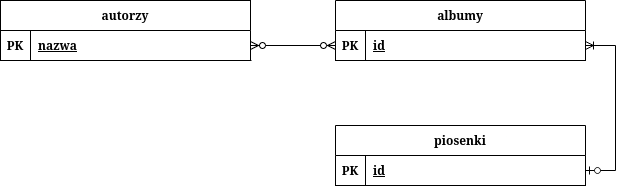
\includegraphics[width=1\textwidth]{images/ch3-db-relacje.drawio.png}
	\caption{\centering{Model relacji bazy}}
	\label{fig:dbrelations}
\end{figure}

Na rysunku nr.~\ref{fig:dbrelations} ukazany jest uproszczony model bazy danych, biorący tylko pod uwagę komponenty potrzebne do określenia relacji. Autorzy są w relacji $M$ do $N$ z albumami. Każdy autor może mieć wiele albumów, a każdy album wiele autorów. Piosenki z albumami są w relacji $1$ do $N$. Każda piosenka może należeć wyłącznie do jednego albumu, ale każdy album może mieć wiele piosenek.

Warto zauważyć, że piosenki niebezpośrednio łączą się z autorami. Jeżeli piosenka chce uzyskać swojego autora, musi zrobić to poprzez album.
